\documentclass{beamer}
\usetheme{Madrid}
\usecolortheme{default}

\usepackage[T1]{fontenc}
\usepackage{lmodern}
\usepackage{booktabs}
\usepackage{tabularx}
\usepackage{siunitx}
\usepackage{tikz}
\usepackage{pgfplots}
\pgfplotsset{compat=1.18}
\usetikzlibrary{arrows.meta,positioning}

% --- Custom colors and styling ---
\definecolor{uoftblue}{RGB}{6,41,88}
\setbeamercolor{titlelike}{bg=uoftblue, fg=white}
\setbeamerfont{title}{series=\bfseries}
\setbeamertemplate{navigation symbols}{} % remove nav symbols

\newcommand{\catchR}{\SI{0.22}{\metre}}
\newcommand{\bestMiss}{\SI{0.62}{\metre}}

% --- Metadata ---
\title[Dynamic Object Capture]
{Dynamic Object Detection \& Capture for UAVs}

\subtitle{Aerial Robotics Club Summer Research}

\author[Terry Yang, Tommy Yang \& Felicia Zhou]
{Terry Yang, Tommy Yang \& Felicia Zhou}

\institute[UTIAS]
{
  University of Toronto Institute for Aerospace Studies \\
  Aerial Robotics Club Summer Research Program
}

\date[Wednesday, August 20, 2025]
{Tuesday, August 25, 2026}

\logo{
\includegraphics[height=0.8cm]{logo_uoft}}

% ------------------------------
\begin{document}

% --- Title Slide ---
\frame{\titlepage}

% --- Outline ---
\begin{frame}
\frametitle{Outline}
\tableofcontents
\end{frame}

% ==============================
\section{Introduction}

\begin{frame}
\frametitle{Problem Definition}
\begin{itemize}
    \item Unmanned aerial vehicles (UAVs) are becoming increasingly important and active within multidisciplinary applications
    \item \textbf{Dynamic object capture} aligns with the current trend to increase levels of autonomy and productivity in today’s society
    \item A complex multi-stage challenge including tracking, detection, trajectory planning, interception, and capture
    \item Existing UAV object-interaction research often focuses on stationary objects and robotic grasping mechanisms in controlled environments
\end{itemize}
\end{frame}

\begin{frame}
\frametitle{Goal and Objectives}
\begin{itemize}
    \item Build the full chain---\textbf{detect, range, frame, filter, plan}---from a single camera to a reachable catch, addressing tracking latency and true ballistic (freefall) intercept
    \item Use Gazebo / SIL as a \textbf{staged verification} of that loop before hardware; keep filter and planner transferable to a real flight stack
    \item On the aircraft: \textbf{YOLO} for detection and \textbf{PnP} for ranging; simulation may stand in with simpler vision only to close the loop
\end{itemize}
\end{frame}

% ==============================
\section{Related Works}

% \begin{frame}
% \frametitle{Related Works}
% \begin{itemize}
%     \item \textbf{Corsel, C.W. (2020):} Proposed a YOLO-based CNN approach for drone obstacle detection and reviewed its performance.
%     \item \textbf{Jaffari et al. (2021):} Experimentally investigated and evaluated deep learning methods for detecting thin objects, highlighting the need for more reliable approaches.
%     \item \textbf{Zhou et al. (2017):} Developed and implemented an edge extraction and enhancement method specifically for fast and accurate thin-structure detection.
% \end{itemize}
% \end{frame}

\begin{frame}
\frametitle{Related Works}
\textbf{“A Real-Time Method to Detect and Track Moving Objects (DATMO) from Unmanned Aerial Vehicles (UAVs) Using a Single Camera” by Rodríguez-Canosa et al.} 
\begin{itemize}
    \item Estimated camera motion is used to calculate an artificial optical flow, which is compared to the real optical flow to differentiate dynamic objects from static objects
    \item Complexity of recording process will contribute to detection and tracking latencies
\end{itemize}
\end{frame}


\begin{frame}
\frametitle{Related Works}
\textbf{“Autonomous drone with ability to track and capture an aerial target” by García et al.} 
\begin{itemize}
    \item A large net was placed on top of a frame built around the UAV to maximize the area of capture 
    \item Ball was not in freefall which may impact orientation of the net and general structure built around the UAV
\end{itemize}
\end{frame}


% ==============================
\section{Methodology}

\begin{frame}
\frametitle{Physical Setup}
\centering
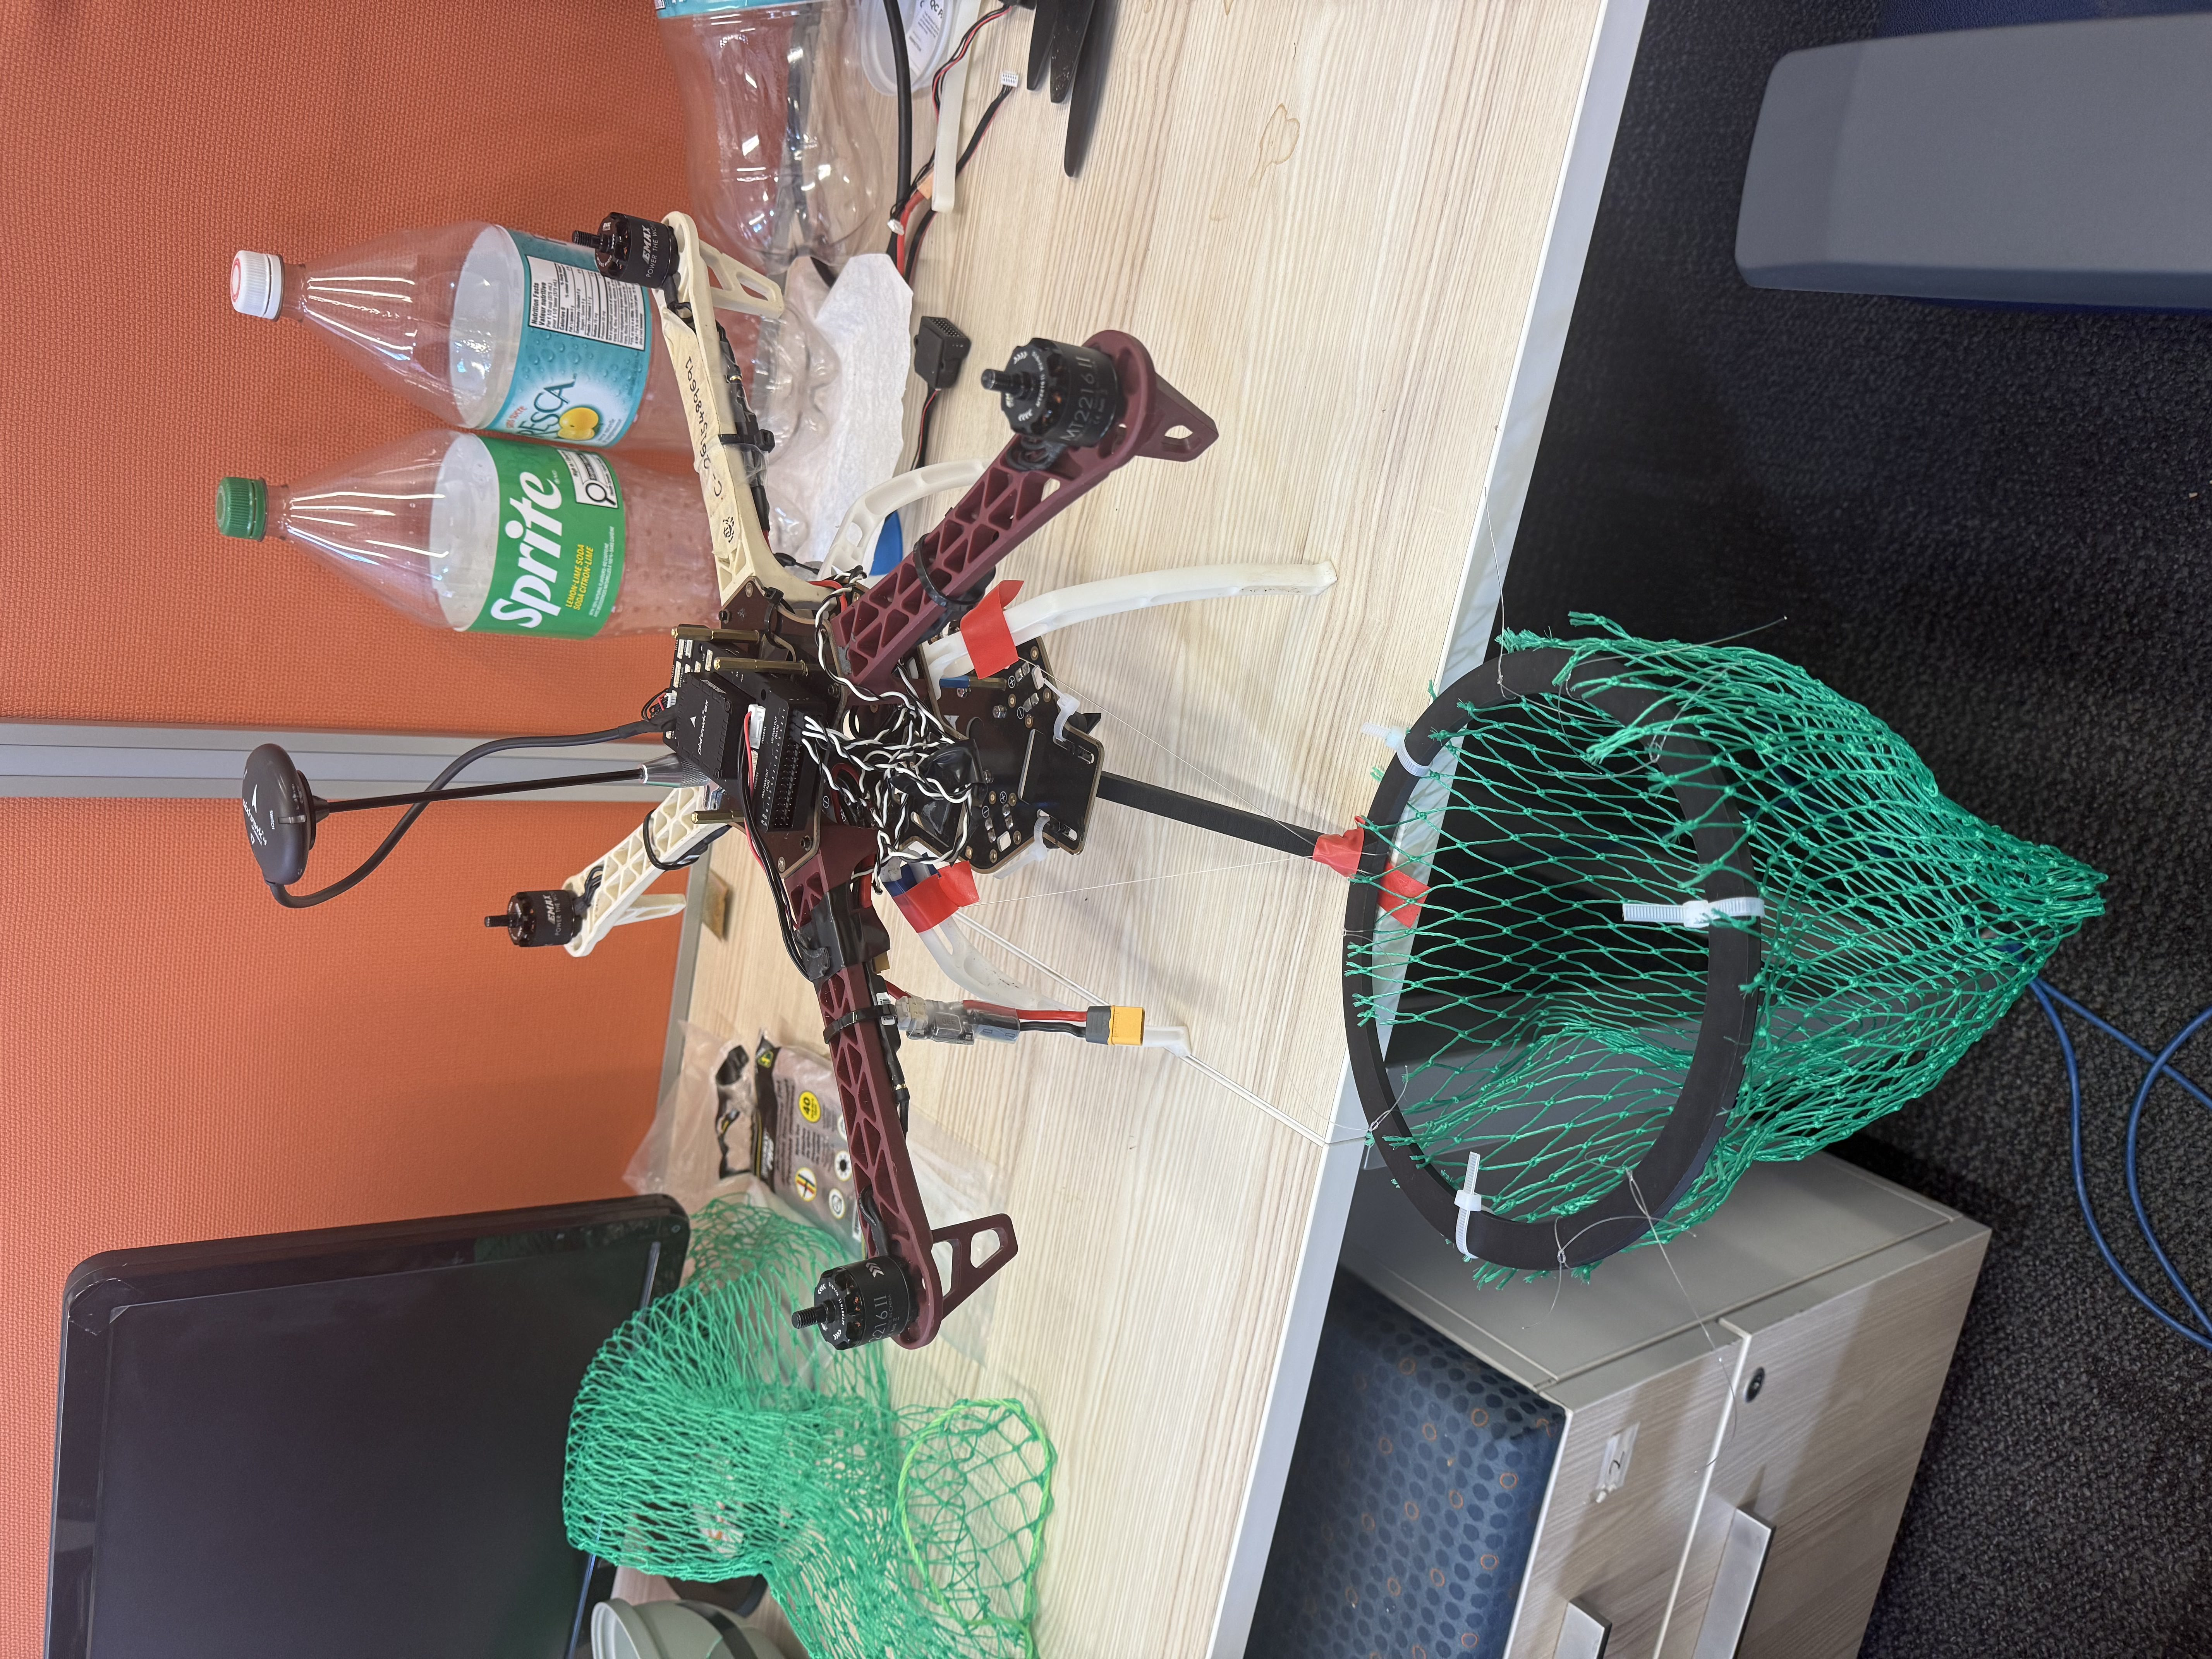
\includegraphics[width=0.95\textwidth,height=0.78\textheight,keepaspectratio]{physical_design.jpg}
\end{frame}

\begin{frame}
\frametitle{Closed-Loop Intercept Stack}
\centering
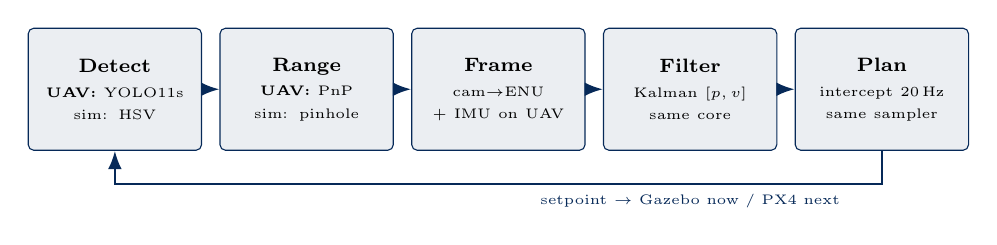
\begin{tikzpicture}[
    font=\scriptsize,
    box/.style={draw=uoftblue, rounded corners=2pt, align=center,
                inner sep=4pt, fill=uoftblue!8, minimum height=1.55cm, text width=1.92cm},
    arr/.style={-{Latex}, thick, uoftblue}
  ]
  \node[box] (d) {\textbf{Detect}\\[1pt]{\tiny\textbf{UAV:} YOLO11s}\\{\tiny sim: HSV}};
  \node[box, right=0.22cm of d] (r) {\textbf{Range}\\[1pt]{\tiny\textbf{UAV:} PnP}\\{\tiny sim: pinhole}};
  \node[box, right=0.22cm of r] (f) {\textbf{Frame}\\[1pt]{\tiny cam$\to$ENU}\\{\tiny + IMU on UAV}};
  \node[box, right=0.22cm of f] (k) {\textbf{Filter}\\[1pt]{\tiny Kalman $[p,v]$}\\{\tiny same core}};
  \node[box, right=0.22cm of k] (p) {\textbf{Plan}\\[1pt]{\tiny intercept 20\,Hz}\\{\tiny same sampler}};
  \draw[arr] (d) -- (r);
  \draw[arr] (r) -- (f);
  \draw[arr] (f) -- (k);
  \draw[arr] (k) -- (p);
  \draw[arr] (p.south) -- ++(0,-0.42) -| node[very near start,below,font=\tiny]
    {setpoint $\to$ Gazebo now / PX4 next} (d.south);
\end{tikzpicture}

\vspace{0.55em}
{\small Gazebo+SIL = staged close of the loop. Catch if $\|\mathrm{net}-\mathrm{ball}\|<\catchR$, $z>\SI{0.4}{\metre}$.}
\end{frame}

\begin{frame}
\frametitle{Detect and Range}
\begin{columns}[T]
\begin{column}{0.52\textwidth}
\centering
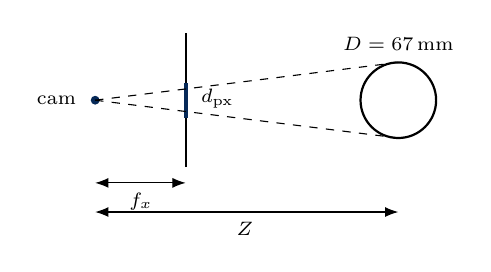
\begin{tikzpicture}[font=\scriptsize, >=Latex]
  \fill[uoftblue] (0,0) circle (1.6pt);
  \node[left] at (-0.12,0) {cam};
  \draw[thick] (1.15,-0.85) -- (1.15,0.85);
  \draw[uoftblue, line width=1.6pt] (1.15,-0.22) -- (1.15,0.22);
  \node[right] at (1.22,0.02) {$d_{\mathrm{px}}$};
  \draw[thick] (3.85,0) circle (0.48);
  \node at (3.85,0.72) {$D=67$\,mm};
  \draw[dashed] (0,0) -- (3.85,0.48);
  \draw[dashed] (0,0) -- (3.85,-0.48);
  \draw[{Latex}-{Latex}] (0,-1.05) -- (1.15,-1.05);
  \node[below] at (0.58,-1.05) {$f_x$};
  \draw[{Latex}-{Latex}] (0,-1.42) -- (3.85,-1.42);
  \node[below] at (1.9,-1.42) {$Z$};
\end{tikzpicture}
\vspace{0.15em}

{\small $Z = 0.067\cdot f_x / d_{\mathrm{px}}$\quad(sim stand-in)}
\end{column}
\begin{column}{0.46\textwidth}
\centering
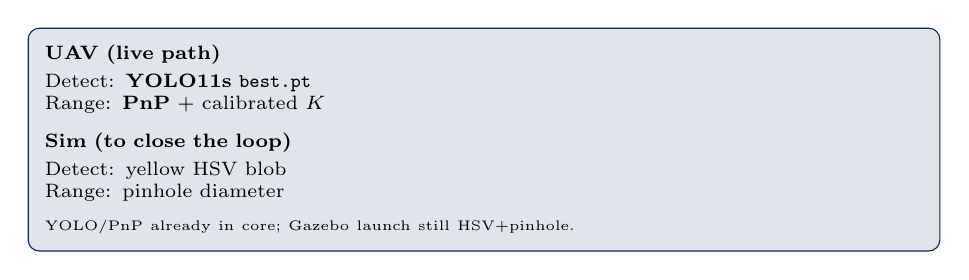
\begin{tikzpicture}[font=\scriptsize]
  \node[draw=uoftblue, fill=uoftblue!12, rounded corners, align=left,
        inner sep=6pt, text width=0.92\textwidth] {
    \textbf{UAV (live path)}\\[2pt]
    Detect: \textbf{YOLO11s} \texttt{best.pt}\\
    Range: \textbf{PnP} + calibrated $K$\\[6pt]
    \textbf{Sim (to close the loop)}\\[2pt]
    Detect: yellow HSV blob\\
    Range: pinhole diameter\\[4pt]
    {\tiny YOLO/PnP already in core; Gazebo launch still HSV+pinhole.}
  };
\end{tikzpicture}
\end{column}
\end{columns}
\end{frame}

\begin{frame}
\frametitle{Filter, Plan, Throw}
\begin{columns}[T]
\begin{column}{0.50\textwidth}
\centering
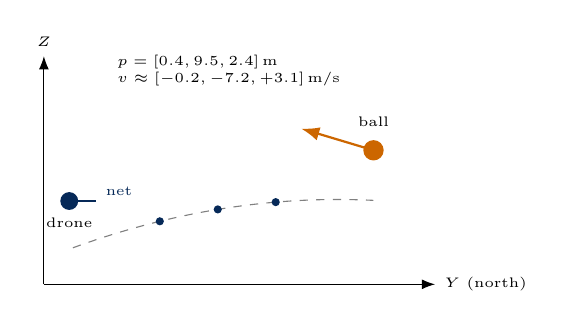
\begin{tikzpicture}[font=\tiny, >=Latex, scale=0.92]
  \draw[->] (0,0) -- (5.4,0) node[right] {$Y$ (north)};
  \draw[->] (0,0) -- (0,3.15) node[above] {$Z$};
  \fill[uoftblue] (0.35,1.15) circle (3.5pt);
  \node[below] at (0.35,1.05) {drone};
  \draw[uoftblue, thick] (0.35,1.15) -- (0.72,1.15);
  \node[right,uoftblue] at (0.72,1.28) {net};
  \fill[orange!80!black] (4.55,1.85) circle (4pt);
  \draw[orange!80!black, thick, ->] (4.55,1.85) -- (3.55,2.15);
  \node[above] at (4.55,2.05) {ball};
  \draw[gray, dashed, domain=0.4:4.55, samples=40]
    plot (\x, {0.35+1.7*\x/4.2 - 0.22*(\x/4.2)*(\x/4.2)*4});
  \foreach \x in {1.6, 2.4, 3.2}
    {\fill[uoftblue] (\x,{0.35+1.7*\x/4.2 - 0.22*(\x/4.2)*(\x/4.2)*4}) circle (1.6pt);}
  \node[align=left] at (2.55,2.95) {$p=[0.4,9.5,2.4]$\,m\\$v\approx[-0.2,-7.2,+3.1]$\,m/s};
\end{tikzpicture}
\end{column}
\begin{column}{0.48\textwidth}
\vspace{-0.2em}
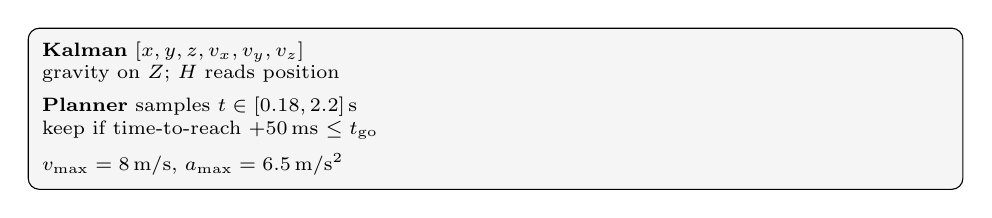
\begin{tikzpicture}[font=\scriptsize]
  \node[draw, rounded corners, fill=black!4, align=left, inner sep=5pt, text width=0.95\textwidth] {
    \textbf{Kalman} $[x,y,z,v_x,v_y,v_z]$\\
    gravity on $Z$; $H$ reads position\\[4pt]
    \textbf{Planner} samples $t\in[0.18,2.2]$\,s\\
    keep if time-to-reach $+50$\,ms $\leq t_{\mathrm{go}}$\\[4pt]
    $v_{\max}=8$\,m/s, $a_{\max}=6.5$\,m/s$^2$
  };
\end{tikzpicture}
\end{column}
\end{columns}
\end{frame}

% ==============================
\section{Results}

\begin{frame}
\frametitle{Gazebo Demo}
\centering
\href{run:gazebo_demo.mp4}{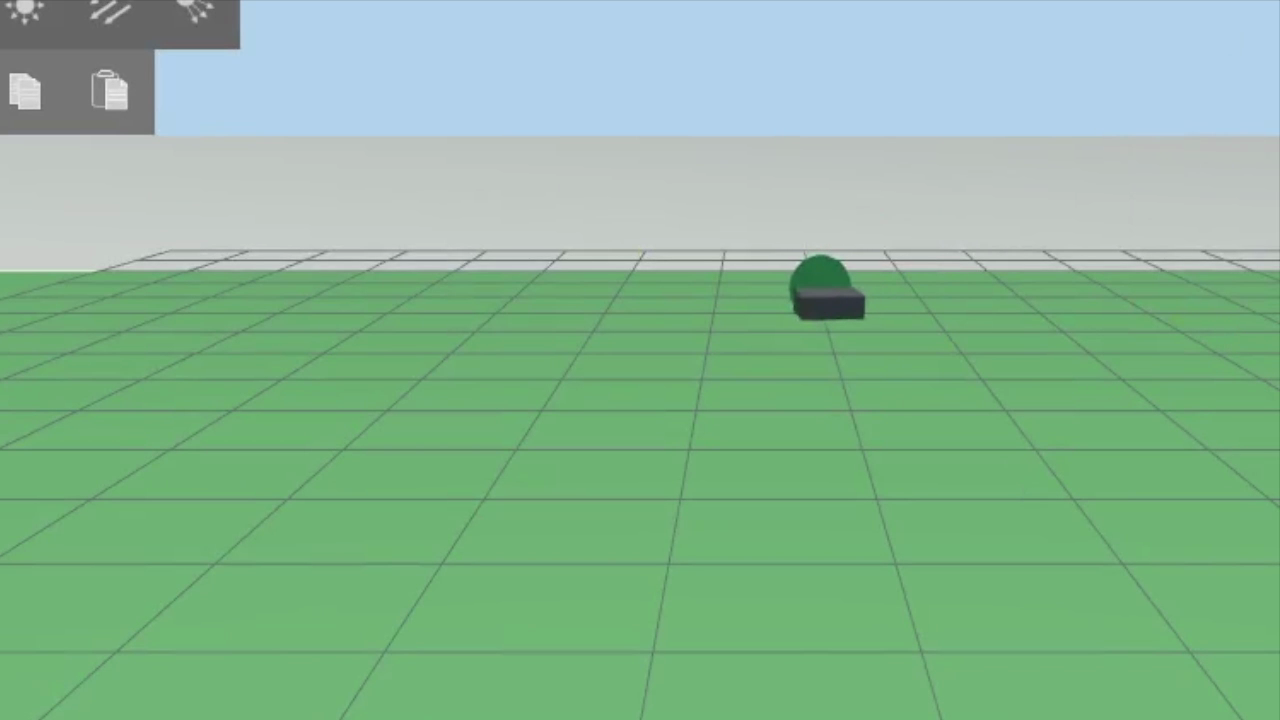
\includegraphics[width=0.95\textwidth,height=0.70\textheight,keepaspectratio]{gazebo_demo_frame.png}}\\[0.35em]
{\small Click the frame to play \texttt{gazebo\_demo.mp4}}
\end{frame}

\begin{frame}
\frametitle{Staged Sim Results}
\begin{columns}[T]
\begin{column}{0.62\textwidth}
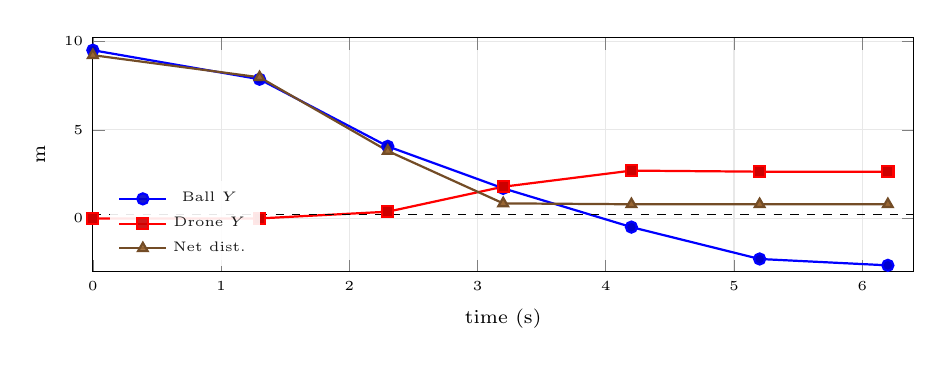
\begin{tikzpicture}
\begin{axis}[
    width=0.99\textwidth, height=4.55cm,
    xlabel={time (s)},
    ylabel={m},
    xmin=0, xmax=6.4, ymin=-3, ymax=10.2,
    legend style={font=\tiny, at={(0.02,0.02)}, anchor=south west, draw=none, fill=white, fill opacity=0.9},
    grid=major, grid style={gray!18},
    tick label style={font=\tiny},
    label style={font=\scriptsize},
  ]
  \addplot+[thick, mark=*] coordinates {
    (0.0,9.5) (1.3,7.86) (2.3,4.07) (3.2,1.7) (4.2,-0.49) (5.2,-2.29) (6.2,-2.65)};
  \addlegendentry{Ball $Y$}
  \addplot+[thick, mark=square*] coordinates {
    (0.0,0.0) (1.3,0.0) (2.3,0.38) (3.2,1.79) (4.2,2.7) (5.2,2.64) (6.2,2.64)};
  \addlegendentry{Drone $Y$}
  \addplot+[thick, mark=triangle*] coordinates {
    (0.0,9.22) (1.3,7.97) (2.3,3.81) (3.2,0.85) (4.2,0.8) (5.2,0.8) (6.2,0.8)};
  \addlegendentry{Net dist.}
  \draw[dashed] (axis cs:0,0.22) -- (axis cs:6.4,0.22);
\end{axis}
\end{tikzpicture}
\end{column}
\begin{column}{0.36\textwidth}
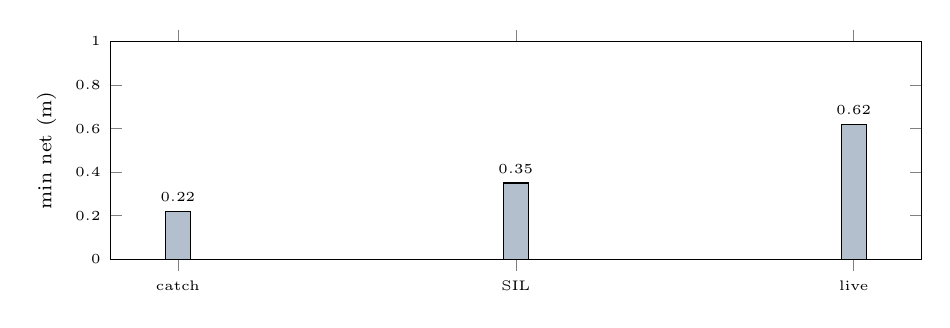
\begin{tikzpicture}
\begin{axis}[
    ybar, bar width=9pt,
    width=0.98\textwidth, height=4.35cm,
    ymin=0, ymax=1.0,
    symbolic x coords={catch, SIL, live},
    xtick=data,
    ylabel={min net (m)},
    tick label style={font=\tiny},
    label style={font=\scriptsize},
    nodes near coords, nodes near coords align={vertical},
    every node near coord/.style={font=\tiny},
  ]
  \addplot[fill=uoftblue!30] coordinates {(catch,0.22) (SIL,0.35) (live,0.62)};
\end{axis}
\end{tikzpicture}
\vspace{0.15em}
{\scriptsize 8/8 tests. SIL catches. Live 0.62--0.80\,m.}
\end{column}
\end{columns}
\end{frame}

% ==============================
\section{Discussion}

\begin{frame}
\frametitle{From Sim Residual to Flight}
\centering
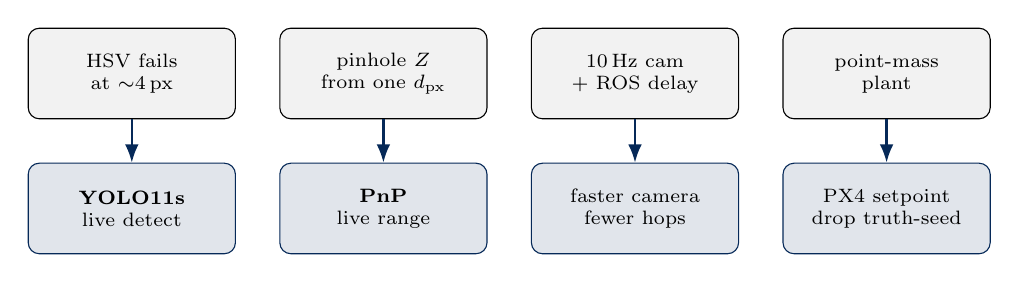
\begin{tikzpicture}[
    font=\scriptsize,
    gap/.style={draw, rounded corners, align=center, inner sep=4pt,
                fill=black!5, text width=2.35cm, minimum height=1.15cm},
    fix/.style={draw=uoftblue, rounded corners, align=center, inner sep=4pt,
                fill=uoftblue!12, text width=2.35cm, minimum height=1.15cm},
    arr/.style={-{Latex}, thick, uoftblue}
  ]
  \node[gap] (g1) {HSV fails\\at $\sim$4\,px};
  \node[gap, right=0.55cm of g1] (g2) {pinhole $Z$\\from one $d_{\mathrm{px}}$};
  \node[gap, right=0.55cm of g2] (g3) {10\,Hz cam\\+ ROS delay};
  \node[gap, right=0.55cm of g3] (g4) {point-mass\\plant};
  \node[fix, below=0.55cm of g1] (f1) {\textbf{YOLO11s}\\live detect};
  \node[fix, below=0.55cm of g2] (f2) {\textbf{PnP}\\live range};
  \node[fix, below=0.55cm of g3] (f3) {faster camera\\fewer hops};
  \node[fix, below=0.55cm of g4] (f4) {PX4 setpoint\\drop truth-seed};
  \draw[arr] (g1) -- (f1);
  \draw[arr] (g2) -- (f2);
  \draw[arr] (g3) -- (f3);
  \draw[arr] (g4) -- (f4);
\end{tikzpicture}

\vspace{0.7em}
{\small Loop works at 30\,Hz (SIL catch). Next: YOLO+PnP on the aircraft, same filter and planner.}
\end{frame}

\begin{frame}
\frametitle{Future Work}

\begin{itemize}
    \item Test the system under different and more realistic environmental conditions, including wind and varying target velocities
    \item Develop capture mechanisms specific to certain disciplinary applications
    \begin{itemize}
        \item Catching flying balls before they hit spectators in sports games
        \item Preventing falling tools or debris on construction sites from causing head injuries
        \item Mid-air retrieval of rocket when other forms of landing are infeasible
    \end{itemize}
\end{itemize}

\end{frame}


% ==============================
\section{Acknowledgements}

\begin{frame}
\frametitle{Acknowledgements}
We would like to express our sincere gratitude to the ARC program at UTIAS for providing this invaluable research opportunity. We are thankful to Prof. Liu, the faculty members, and all the graduate students for their support and insightful guidance throughout the program. We are especially grateful to Kevin for his continuous mentorship and exceptional teaching; his contributions have made this experience deeply educational and truly eye-opening.
\end{frame}

% --- Final Slide ---
\begin{frame}
\centering
\Huge \textbf{Thank You!} \\
\vspace{0.5cm}
\large Questions?
\end{frame}

\end{document}
